
\documentclass[10pt]{article}
\usepackage[utf8]{inputenc}
\usepackage{graphicx}
\usepackage{amsmath, amssymb}
\usepackage{geometry}
\usepackage{caption} 
\geometry{a4paper, margin=0.5in, landscape} 

\begin{document}

\section*{Comparative EIS Kinetics Report}
\textbf{Model Structure:} \texttt{R0-p(R1-p(R2-Ws2,CPE2),CPE1)}

\begin{center}
    \includegraphics[width=0.45\textwidth]{circuit_2RC_Ws.png}
\end{center}

\renewcommand{\arraystretch}{1.6} 
\begin{table}[h!]
    \centering
    \footnotesize
    \begin{tabular}{|l|c|c|c|c|c|c|c|}
        \hline
        \textbf{Element} & \textbf{Unit} & \textbf{Bounds} & \textbf{Cauvel\_3\_Mo\_8H} & \textbf{Cauvel\_3\_Mo\_24H} & \textbf{Cauvel\_3\_Mo\_48H} & \textbf{Cauvel\_3\_Mo\_72H} & \textbf{Cauvel\_3\_Mo\_168H} \\ \hline
        $R_{0}$ & $\Omega$ & $[1.0e-03, 1.0e+03]$ & $5.47e+01 \pm 3.5e-01$ & $5.50e+01 \pm 3.6e-01$ & $1.09e+01 \pm 6.5e+01$ & $5.28e+01 \pm 3.3e-01$ & $6.12e+01 \pm 3.3e-01$ \\ \hline
        $R_{1}$ & $\Omega$ & $[1.0e+00, 1.0e+08]$ & $5.73e+03 \pm 3.1e+02$ & $6.88e+03 \pm 7.4e+02$ & $4.66e+01 \pm 6.5e+01$ & $8.04e+03 \pm 8.3e+02$ & $4.04e+03 \pm 1.8e+03$ \\ \hline
        $R_{2}$ & $\Omega$ & $[1.0e+00, 1.0e+08]$ & $6.66e+03 \pm 2.0e+03$ & $5.59e+03 \pm 4.5e+03$ & $6.01e+03 \pm 5.4e+02$ & $8.75e+03 \pm 6.9e+03$ & $1.04e+00 \pm 3.5e+05$ \\ \hline
        $W_{2,R}$ & $\Omega$ & $[1.0e-03, 1.0e+07]$ & $1.65e+04 \pm 4.3e+03$ & $1.54e+04 \pm 3.0e+03$ & $2.10e+04 \pm 1.1e+03$ & $1.15e+04 \pm 4.7e+03$ & $1.15e+04 \pm 3.5e+05$ \\ \hline
        $W_{2,\tau}$ & sec & $[1.0e-06, 1.0e+04]$ & $6.87e+01 \pm 2.9e+01$ & $3.37e+01 \pm 8.6e+00$ & $3.44e+01 \pm 2.9e+00$ & $3.46e+01 \pm 1.4e+01$ & $1.07e+00 \pm 3.7e+01$ \\ \hline
        $Q_{2}$ & $\Omega$$^{-1}$ sec$^{a}$ & $[1.0e-09, 1.0e-03]$ & $3.09e-04 \pm 2.4e-05$ & $2.40e-04 \pm 3.7e-05$ & $1.09e-04 \pm 5.6e-06$ & $3.31e-04 \pm 5.7e-05$ & $4.77e-04 \pm 1.6e-03$ \\ \hline
        $n_{2}$ & - & $[5.0e-01, 1.0e+00]$ & $1.00e+00 \pm 1.0e-01$ & $1.00e+00 \pm 2.5e-01$ & $8.89e-01 \pm 7.2e-03$ & $1.00e+00 \pm 2.3e-01$ & $7.90e-01 \pm 5.5e-01$ \\ \hline
        $Q_{1}$ & $\Omega$$^{-1}$ sec$^{a}$ & $[1.0e-10, 1.0e-03]$ & $7.42e-05 \pm 1.9e-06$ & $9.35e-05 \pm 2.7e-06$ & $5.93e-06 \pm 1.1e-05$ & $1.32e-04 \pm 3.3e-06$ & $1.92e-04 \pm 9.0e-06$ \\ \hline
        $n_{1}$ & - & $[5.0e-01, 1.0e+00]$ & $8.80e-01 \pm 5.2e-03$ & $8.91e-01 \pm 6.3e-03$ & $5.00e-01 \pm 1.4e-01$ & $8.69e-01 \pm 5.7e-03$ & $8.61e-01 \pm 9.3e-03$ \\ \hline
        \textbf{$\chi^2$} & - & -  & $1.088e-03$ & $1.250e-03$ & $8.562e-04$ & $1.153e-03$ & $8.434e-04$ \\ \hline

    \end{tabular}
\end{table}


\newpage
\section*{Analysis Results: 8H}
\begin{center}
    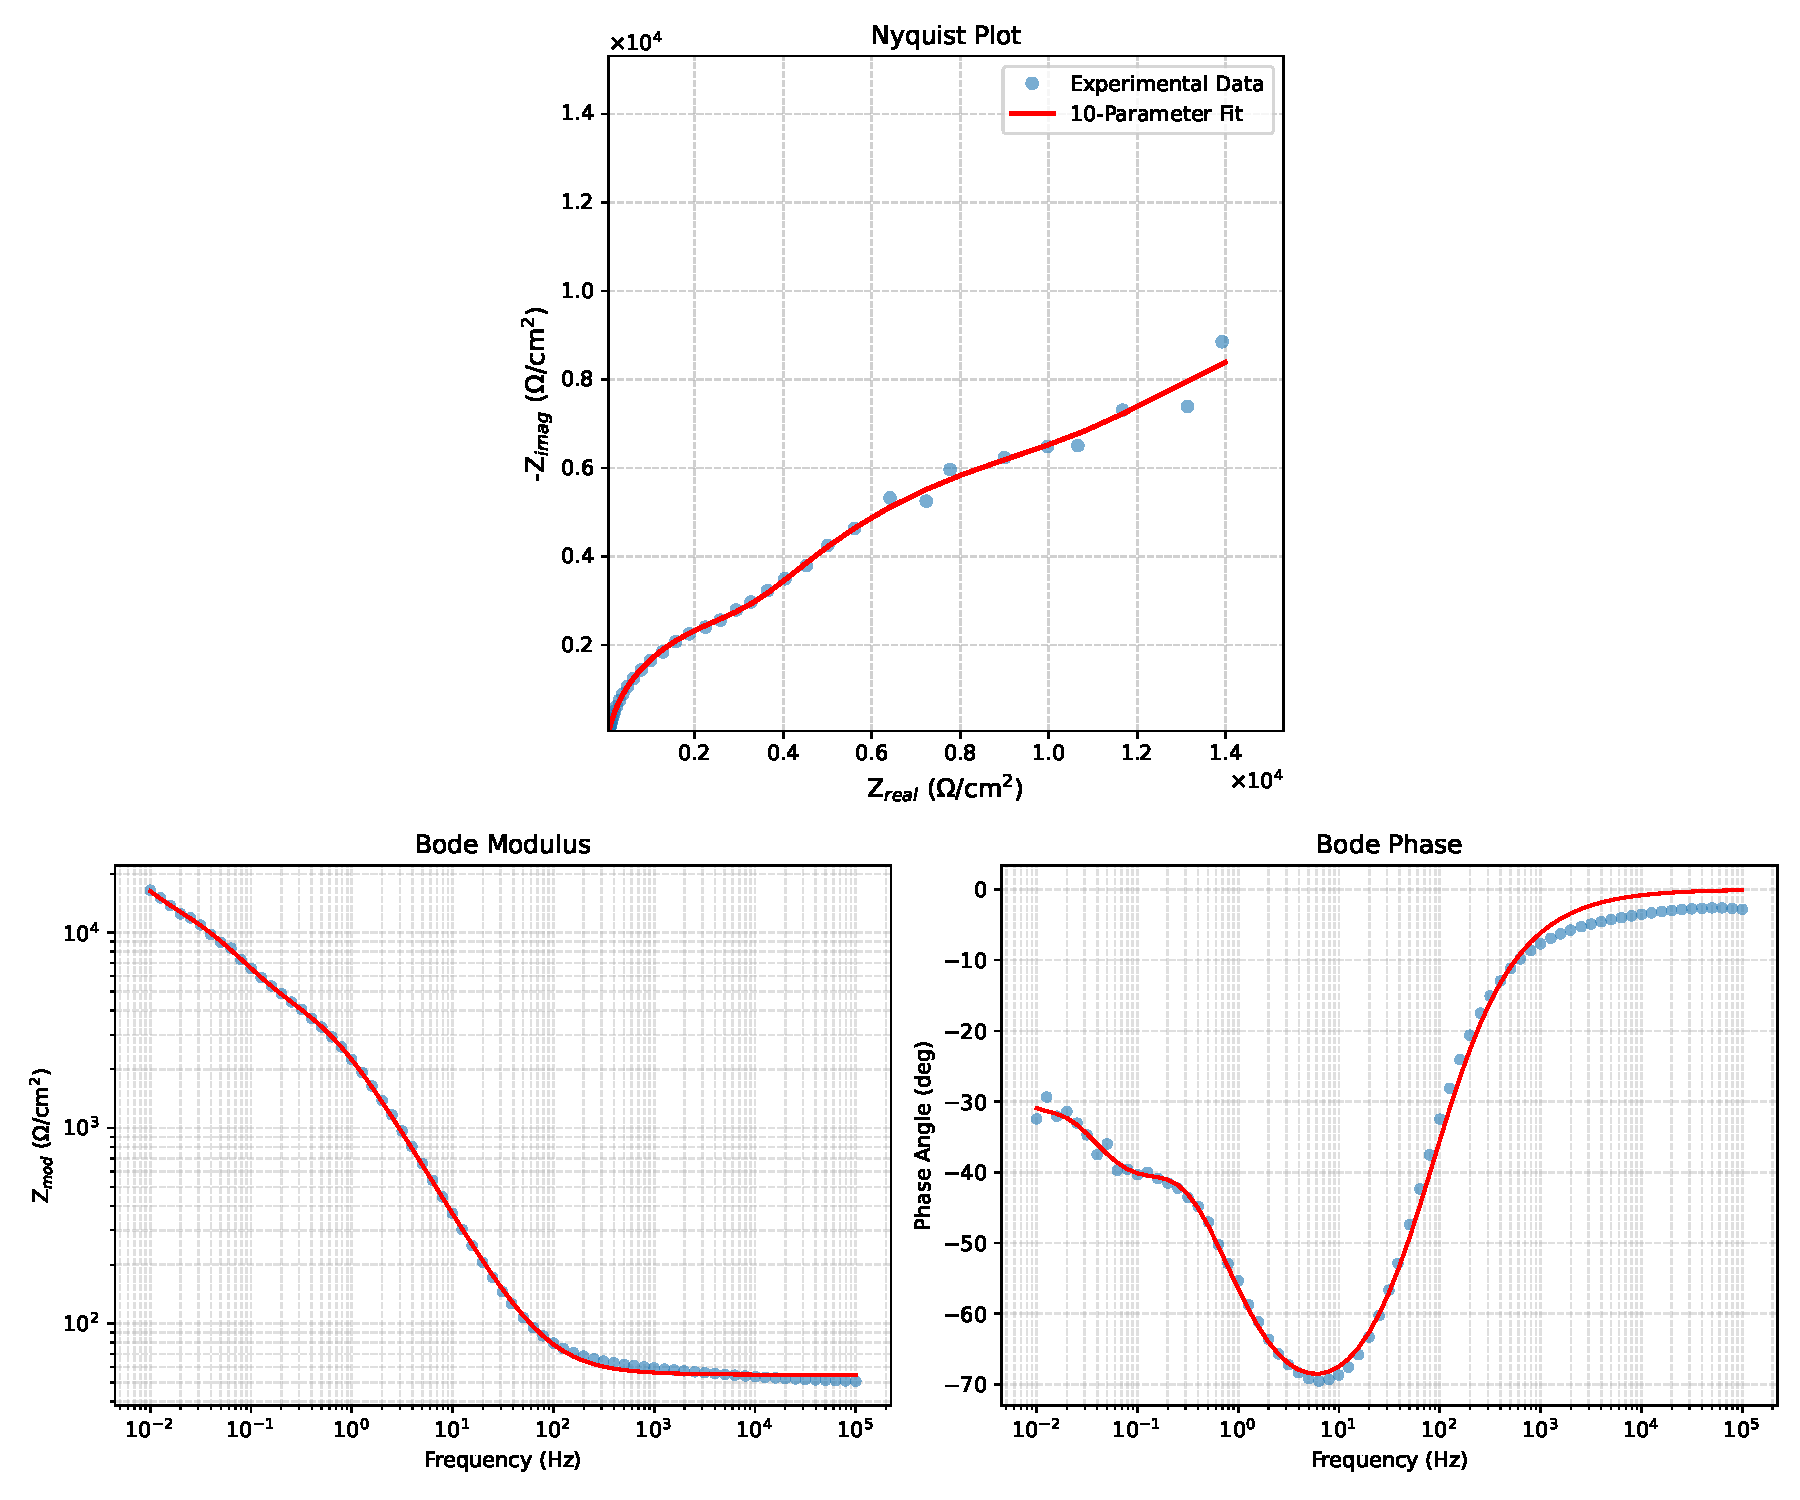
\includegraphics[width=0.7\textwidth]{plots_Cauvel_3_Mo_8H.pdf}
    \captionof{figure}{EIS Fit Results for Cauvel\_3\_Mo\_8H}
\end{center}

\newpage
\section*{Analysis Results: 24H}
\begin{center}
    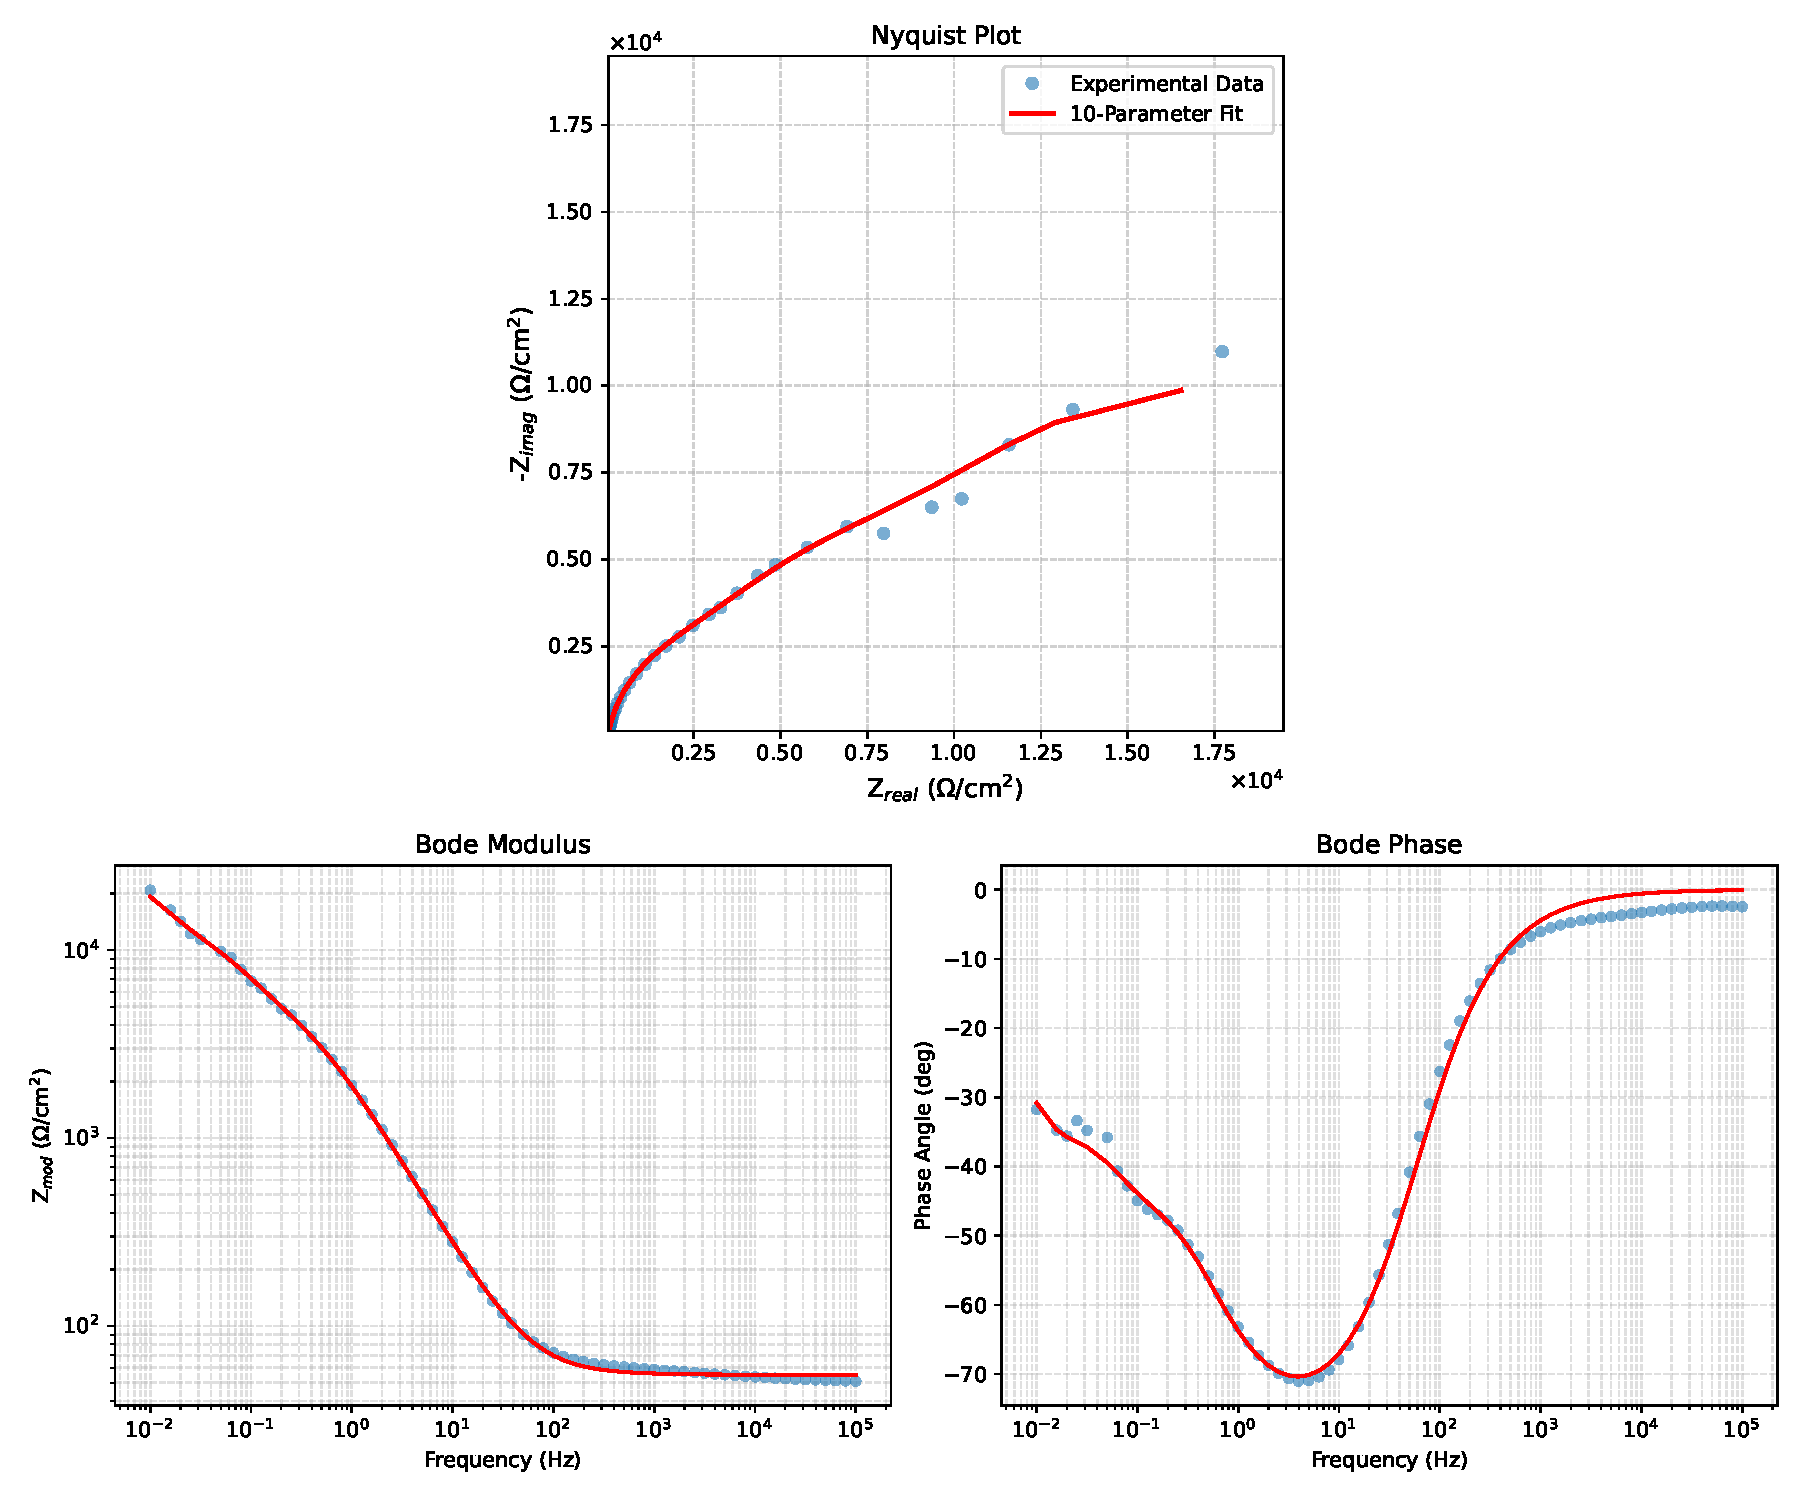
\includegraphics[width=0.7\textwidth]{plots_Cauvel_3_Mo_24H.pdf}
    \captionof{figure}{EIS Fit Results for Cauvel\_3\_Mo\_24H}
\end{center}

\newpage
\section*{Analysis Results: 48H}
\begin{center}
    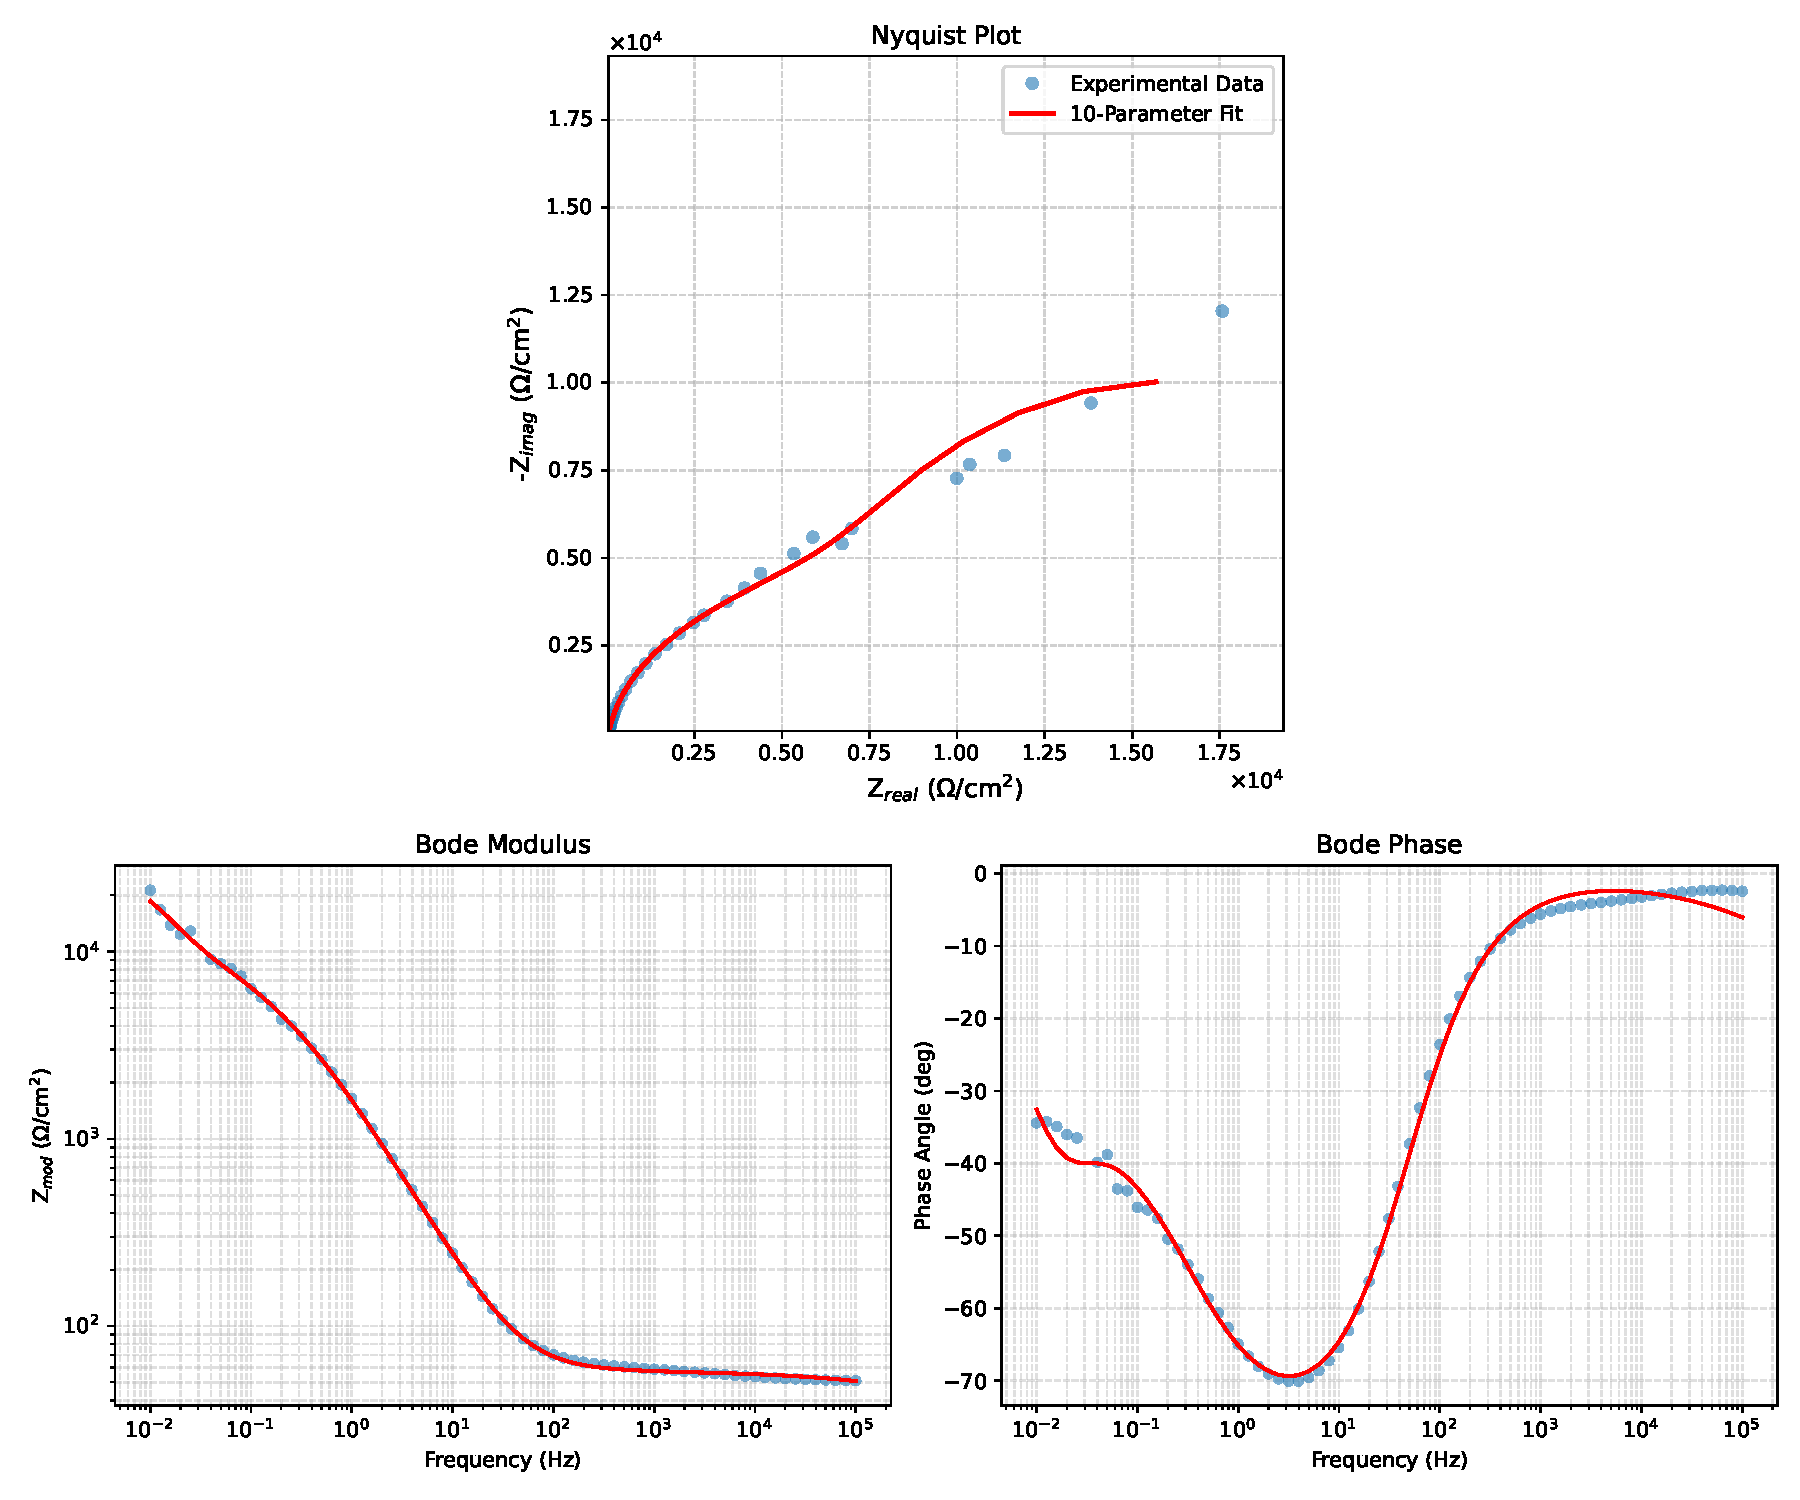
\includegraphics[width=0.7\textwidth]{plots_Cauvel_3_Mo_48H.pdf}
    \captionof{figure}{EIS Fit Results for Cauvel\_3\_Mo\_48H}
\end{center}

\newpage
\section*{Analysis Results: 72H}
\begin{center}
    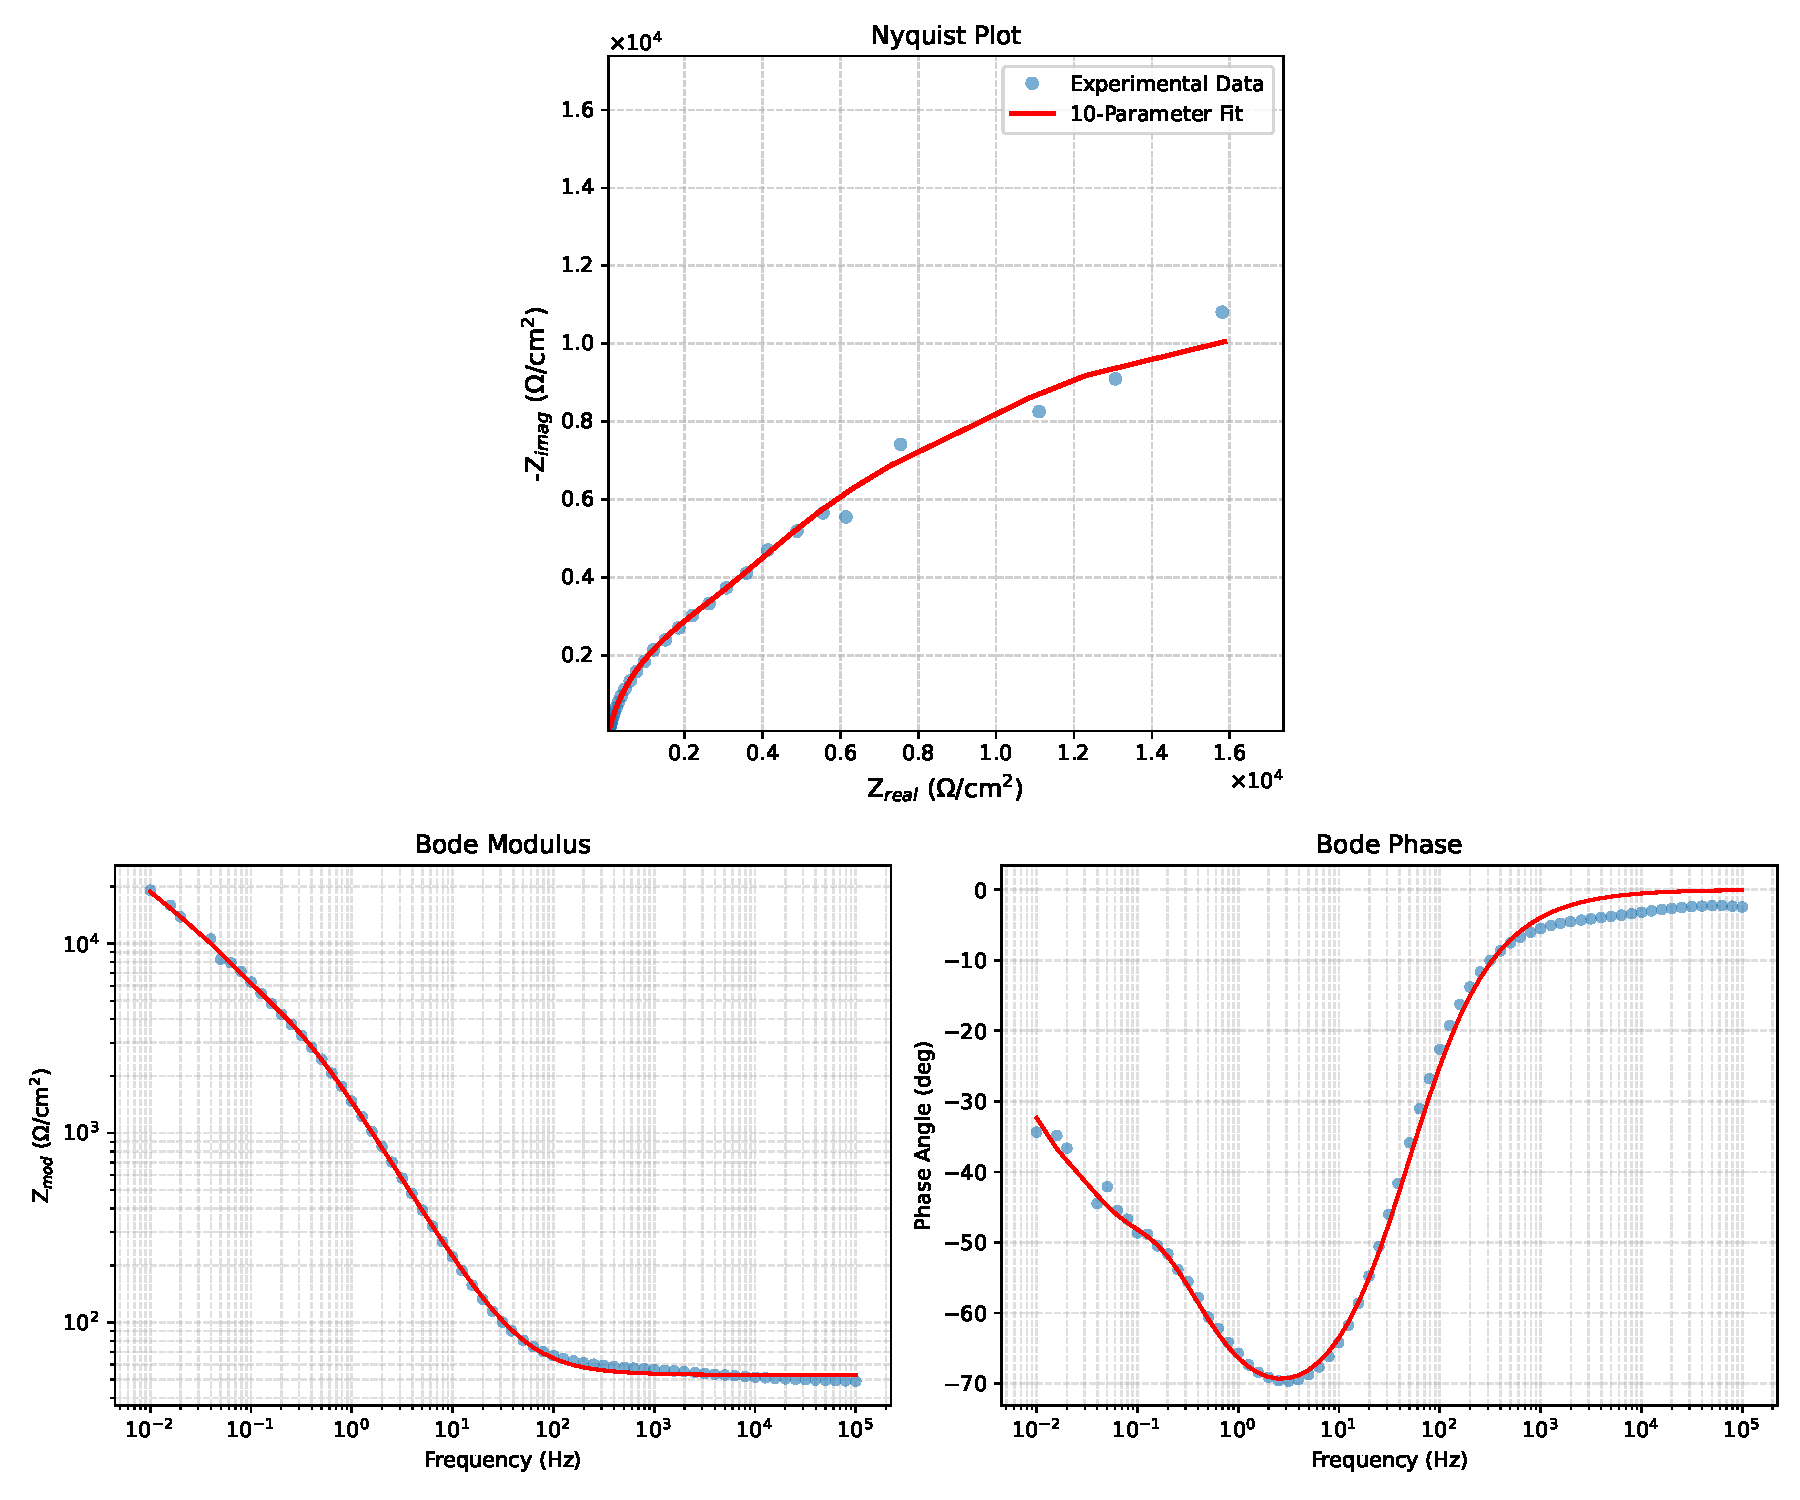
\includegraphics[width=0.7\textwidth]{plots_Cauvel_3_Mo_72H.pdf}
    \captionof{figure}{EIS Fit Results for Cauvel\_3\_Mo\_72H}
\end{center}

\newpage
\section*{Analysis Results: 168H}
\begin{center}
    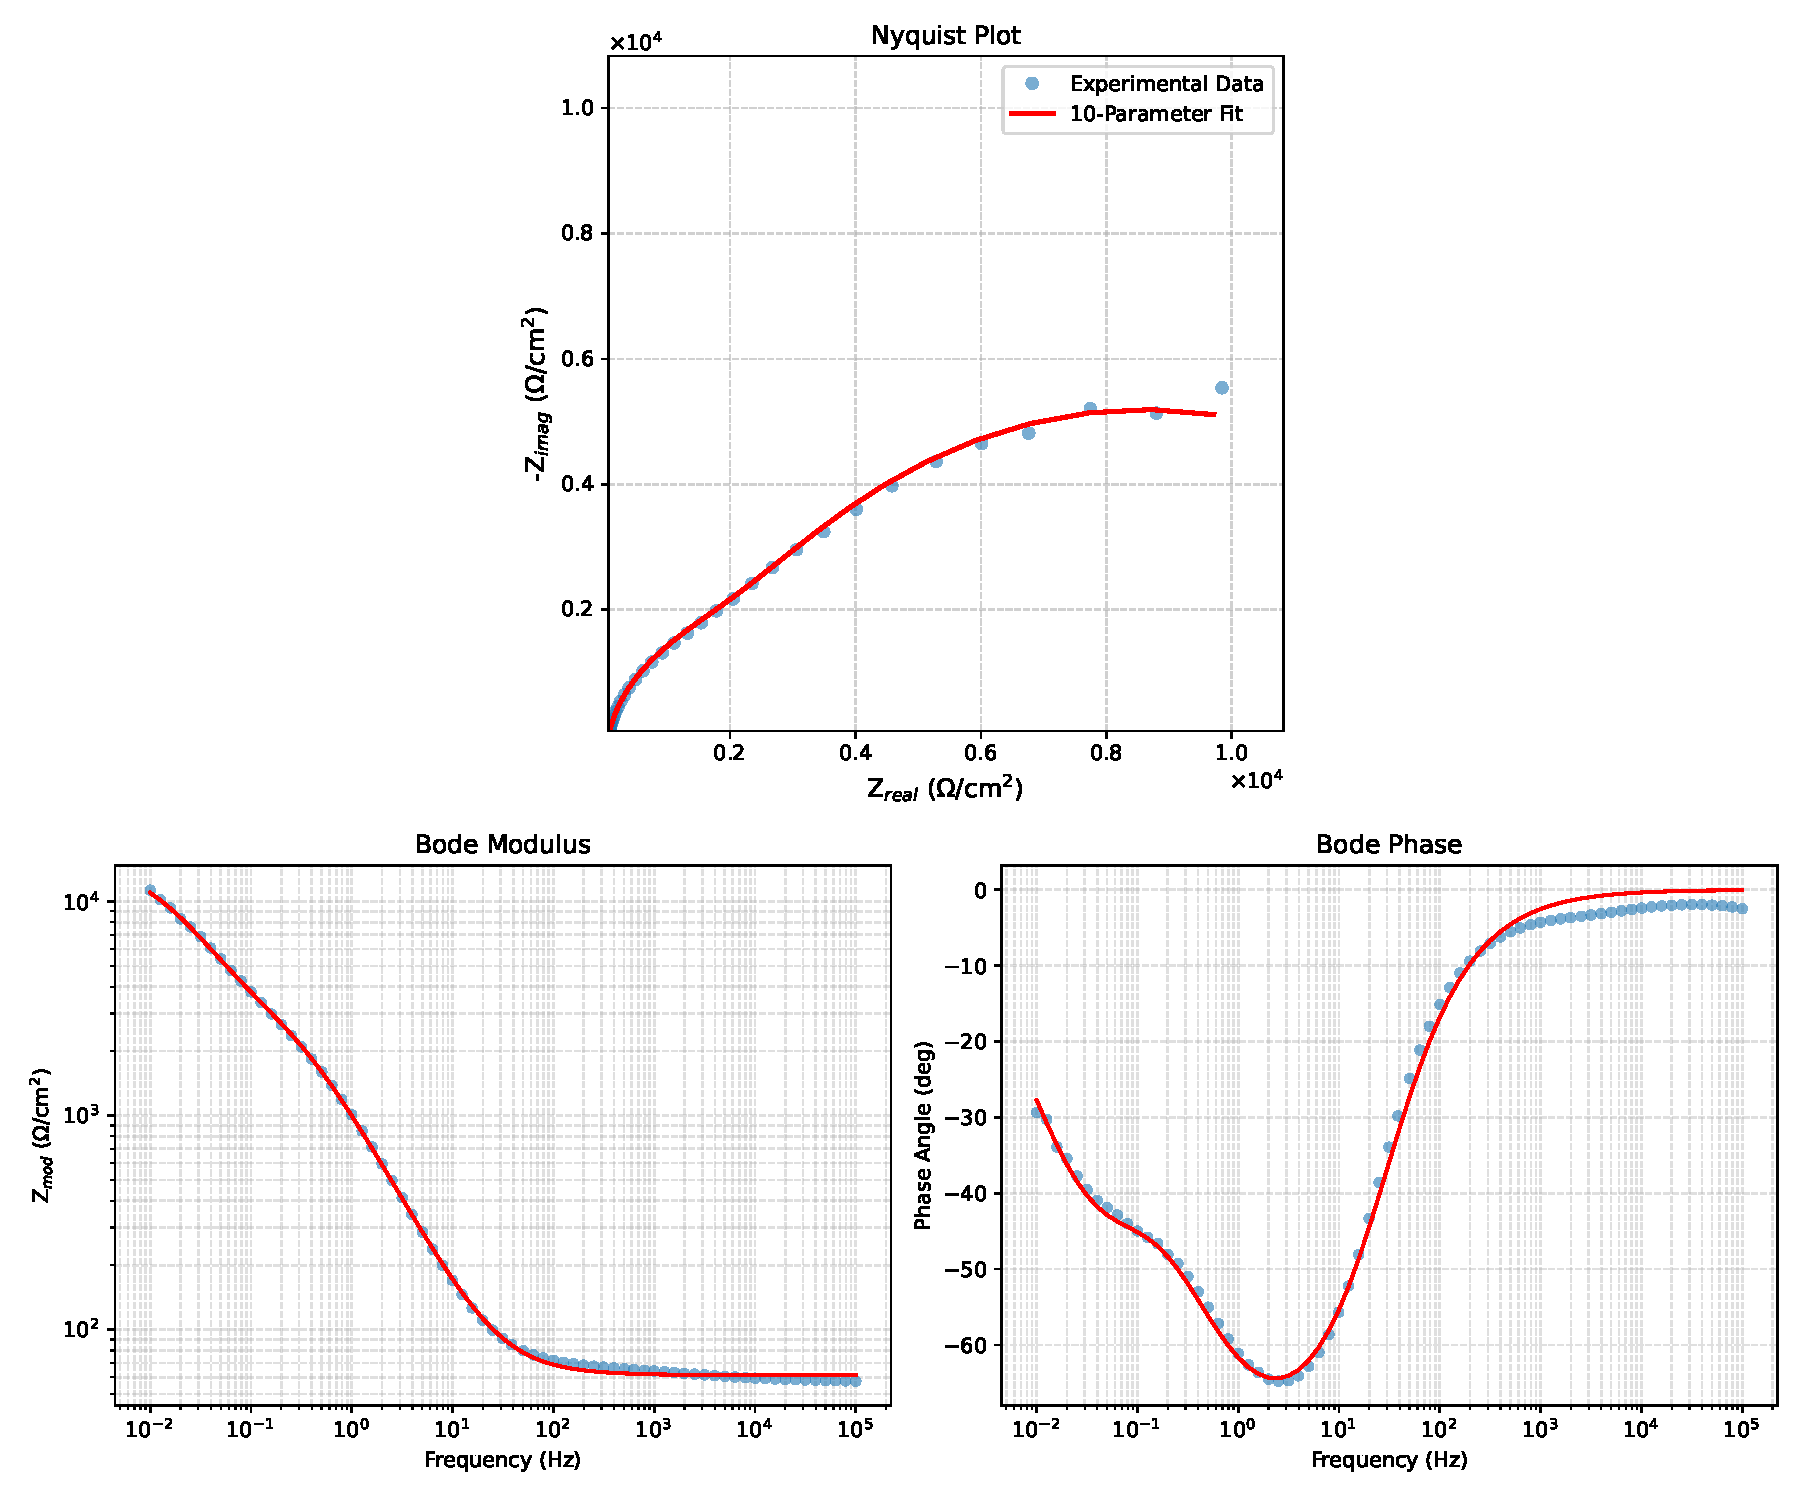
\includegraphics[width=0.7\textwidth]{plots_Cauvel_3_Mo_168H.pdf}
    \captionof{figure}{EIS Fit Results for Cauvel\_3\_Mo\_168H}
\end{center}


\end{document}
